\mode<presentation>
{
  \usetheme{Boadilla}
}

%\usepackage[english]{babel}
\usepackage[utf8]{inputenc}

% Note: using version 2.0-alpha3
\usepackage[cache]{minted}
\setminted{frame=single}

% Hour-long talk

\title[Exploring type-directed TDD w/FizzBuzz]{Exploring type-directed, test-driven development}
\subtitle{A case study using FizzBuzz}
\author{Franklin Chen \\ \url{http://franklinchen.com/}}
\date[\href{http://www.pghtechfest.com/}{Pittsburgh TechFest 2014}]{June 7, 2014 \\ \href{http://www.pghtechfest.com/}{Pittsburgh TechFest 2014}}

\subject{Talks}

% Delete this, if you do not want the table of contents to pop up at
% the beginning of each subsection:
%\AtBeginSubsection[]
%{
%  \begin{frame}<beamer>{Outline}
%    \tableofcontents[currentsection,currentsubsection]
%  \end{frame}
%}

\begin{document}

\maketitle

\begin{abstract}
  An expressive static type system is one of the most joyful and
  powerful tools for prototyping, designing, and maintaining
  programs. In this performance-theatrical presentation, I will
  provide a taste of how to use types, in conjunction with tests, to
  drive iterative development of a particular program, the famous
  FizzBuzz problem. We will solve generalizations of this problem,
  changing and adding requirements, to illustrate the pleasures and
  benefits of ``type thinking''.

  The Scala language will be used as the vehicle for this
  demonstration, but the techniques apply immediately to any
  industrial-strength statically typed language, such as Haskell,
  OCaml, F\#, Rust, and most recently, Swift.

  (Note: this presentation will use live human volunteers to play the
  roles of various programming concepts.)
\end{abstract}

\begin{frame}
  \titlepage
\end{frame}

\section*{Outline}

\begin{frame}{Outline}
  \tableofcontents[subsectionstyle=hide]
\end{frame}

% Since this a solution template for a generic talk, very little can
% be said about how it should be structured. However, the talk length
% of between 15min and 45min and the theme suggest that you stick to
% the following rules:  

% - Exactly two or three sections (other than the summary).
% - At *most* three subsections per section.
% - Talk about 30s to 2min per frame. So there should be between about
%   15 and 30 frames, all told.

\section{Introduction}

\subsection{Goals}

\begin{frame}{Goals of this presentation}
  \begin{itemize}
  \item Give a taste of a \alert{practical} software development \alert{process} that is:
    \begin{itemize}
    \item \alert{test}-driven
    \item \alert{type}-directed
    \end{itemize}
  \item Show everything concretely:
    \begin{itemize}
    \item build environment
    \item testing frameworks
    \item all the code
    \end{itemize}
  \item Use \texttt{FizzBuzz} because:
    \begin{itemize}
    \item problem: easy to understand
    \item modifications: easy to understand
    \item fun!
    \end{itemize}
  \item Encourage you to explore further
    \begin{itemize}
    \item Have you heard the news about \href{https://developer.apple.com/swift/}{Swift}?
      
\includegraphics[height=0.75cm]{swift-hero.png}
    \end{itemize}
  \end{itemize}
\end{frame}

\subsection{Test-driven development (TDD)}

\begin{frame}{Test-driven development (TDD)}
  \begin{itemize}
  \item Think.
  \item Write a test that \textcolor{red}{fails}.
  \item Write code until test \textcolor{green}{succeeds}.
  \item Repeat, and \textcolor{green}{refactor} as needed.
  \end{itemize}

  \begin{block}{\href{http://martinfowler.com/articles/is-tdd-dead/}{Is TDD dead?}}
    My answer: No.
  \end{block}
\end{frame}

\subsection{Type systems}

\begin{frame}{Type systems}
  \begin{block}{What is a type system?}
    For this presentation: a \alert{syntactic} method for \alert{proving} the absence of certain program behaviors.
  \end{block}

  \begin{block}{``Debating'' types ``versus'' tests?}
    Let's just use both!
  \end{block}
\end{frame}

\subsection{Poor versus decent type systems}

\begin{frame}{Poor versus decent type systems}
  \begin{block}{Poor type systems}
    \begin{itemize}
      \mode<article|handout>{
        \item (Developed using 1960s-1970s knowledge)
      }
    \item C, C++, Objective C
    \item Java
    \end{itemize}
  \end{block}

  \begin{block}{Decent type systems}
    \begin{itemize}
      \mode<article|handout>{
        \item (Developed using 1980s-1990s knowledge)
      }
    \item ML (\href{http://www.smlnj.org/}{Standard ML}, \href{http://ocaml.org/}{OCaml}, \href{http://fsharp.org/}{F\#}): I first used for work in 1995
    \item \href{http://www.haskell.org/}{Haskell}: I first used for work in 1995
    \item \href{http://www.scala-lang.org/}{Scala}: first released in 2004
    \item \href{http://www.rust-lang.org/}{Rust}: not yet version 1.0
    \item \href{http://developer.apple.com/swift/}{Swift}: announced by Apple on June 2, 2014!
    \end{itemize}
  \end{block}
\end{frame}

\section{Original FizzBuzz problem}

\subsection{Original FizzBuzz problem}

\begin{frame}{Original FizzBuzz problem}
  \begin{block}{FizzBuzz defined}
    Write a program that prints the numbers from 1 to 100.

    But for multiples of three, print ``Fizz'' instead of the number.

    And for the multiples of five, print ``Buzz''.

    For numbers which are multiples of both three and five, print ``FizzBuzz''.
  \end{block}
\end{frame}

\subsection{Starter Scala code: main driver}

\begin{frame}[fragile]{Starter Scala code: main driver}
  \begin{block}{
\includegraphics[height=0.75cm]{scala-logo-red-dark.png}}
    Scala: a modern \alert{object-oriented} and \alert{functional} language.
  \end{block}

  \inputminted{scala}{Main1.scala}

  \begin{itemize}
  \item Type-directed design: separate out effects (such as printing to terminal) from the real work.
  \item Type-directed feedback: compilation fails when something is not implemented yet.
  \end{itemize}
\end{frame}

\subsection{The joys of continuous compilation and testing}

\begin{frame}[fragile]{The joys of continuous compilation and testing}
  \begin{block}{
\includegraphics[height=0.75cm]{sbt-logo-orange-600x360.png}}
    \href{http://www.scala-sbt.org/}{SBT}: build tool supporting Scala, Java\dots
  \end{block}

  \begin{block}{Killer features}
    \begin{itemize}
    \item \href{http://www.scala-sbt.org/release/docs/Detailed-Topics/Triggered-Execution.html}{Source file changes trigger smart recompilation!}
    \item Source file changes trigger rerun of the tests that depend on changed code!
    \end{itemize}
  \end{block}

  \inputminted{console}{testQuick.console}
\end{frame}

\begin{frame}[fragile]{Write type-directed stub}
  \inputminted{scala}{Main2.scala}

  \begin{block}{Write wanted type signature}
    \mintinline{scala}{???} is convenient for stubbing.
    \begin{itemize}
    \item In Scala standard library
    \item Just performs: \mintinline{scala}{throw new NotImplementedError}
    \end{itemize}
  \end{block}
\end{frame}

\subsection{Write acceptance test (simplified)}

\begin{frame}[fragile]{Write acceptance test (simplified)}
  \begin{block}{
\includegraphics[height=0.75cm]{specs2.png}}
    \href{http://specs2.org/}{Specs2}: a fine testing framework for Scala, Java\dots
  \end{block}

  \inputminted{scala}{MainSpec1.scala}

  \mode<article>{
    A realistic acceptance test would involve handling I/O, but an elegant
    technique for modularizing that,
    \href{https://github.com/scalaz/scalaz-stream}{\texttt{scalaz-stream}},
    is outside the scope of this presentation.
  }
\end{frame}

\begin{frame}[fragile]{Test passes type check, but fails}
  Incremental compilation/testing kicks in:

  \inputminted{console}{testQuick2.console}
\end{frame}

\begin{frame}[fragile]{Outside-in: toward a \mintinline{scala}{FizzBuzz} unit}
  Types are shapes to assemble logically.

  \inputminted{scala}{Main4.scala}

  \begin{itemize}
  \item \mintinline{scala}{(start to end): Seq[Int]}, where \href{http://www.scala-lang.org/api/2.11.0/index.html\#scala.collection.Seq}{\mintinline{scala}{Seq[_]}} is a \alert{type constructor} that, given a type \mintinline{scala}{A}, returns a type of \mintinline{scala}{Seq[A]}.
    \pause
  \item For any value of type \mintinline{scala}{Seq[A]}, \mintinline{scala}{map: (A => B) => Seq[B]}.
  \begin{center}
    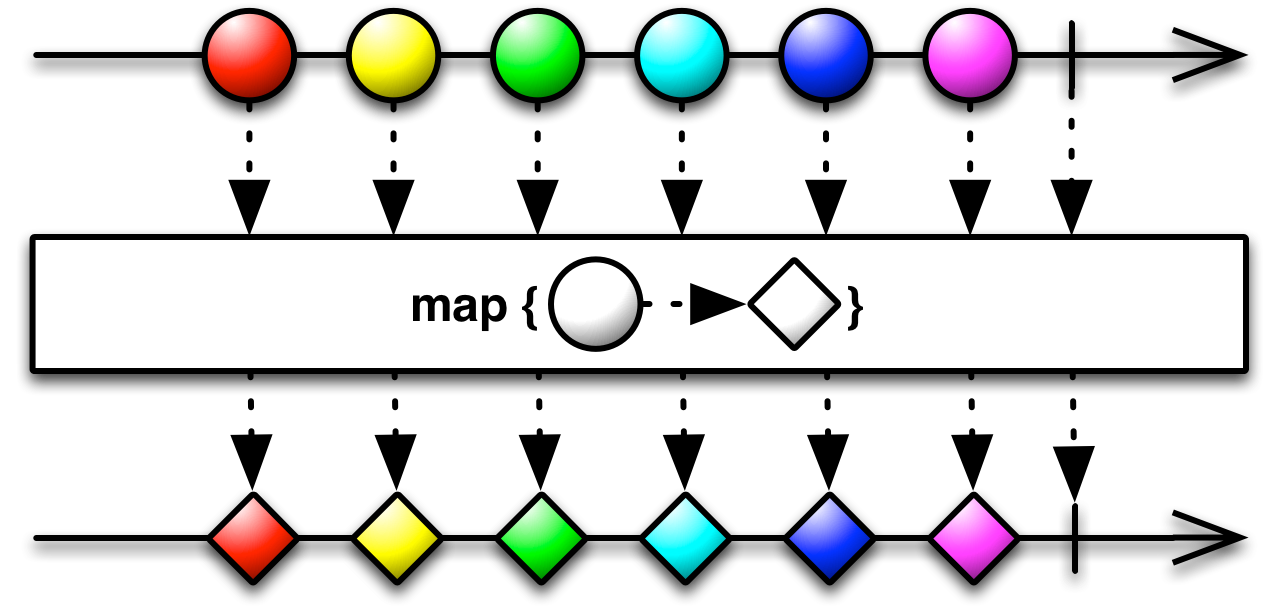
\includegraphics[height=2.5cm]{map.png}
  \end{center}
  \pause
  \item Therefore: need to implement function \mintinline{scala}{FizzBuzz.evaluate: Int => String}.
  \end{itemize}
\end{frame}

\subsection{Test-driven units}

\begin{frame}[fragile]{Start writing the \texttt{FizzBuzz} module}
  A failing acceptance test drives \alert{discovery} of
  \begin{itemize}
  \item A \alert{unit}, \texttt{FizzBuzz}
  \item A function with a particular type,
    \mintinline{scala}{Int => String}
  \end{itemize}

  \inputminted{scala}{FizzBuzz1.scala}

  \begin{block}{\alert{Types} are better than \alert{comments} as \alert{documentation}!}
    Comments are not checkable, unlike types and tests.
  \end{block}
\end{frame}

\begin{frame}[fragile]{First cut at unit tests: example-based}
  \inputminted{scala}{FizzBuzzSpec1.scala}
\end{frame}

\subsection{Property-based tests}

\begin{frame}[fragile]{The joy of property-based tests}
    \begin{block}{
\includegraphics[height=0.75cm]{logo_forall_h61.png}
\includegraphics[height=0.75cm]{logo_scalacheck_h61.png}}
      \href{http://scalacheck.org/}{ScalaCheck}: a framework for writing \alert{property-based} tests.
  \end{block}

  \inputminted{scala}{FizzBuzzSpec2.scala}

  \begin{block}{Killer features}
    \begin{itemize}
    \item Auto-generates random tests for each property (100 by default).
    \item \alert{Type-driven}: here, generates random \mintinline{scala}{Int} values.
    \end{itemize}
  \end{block}
\end{frame}

\begin{frame}[fragile]{Property-based tests (continued)}
  The other three properties of interest:

  \inputminted{scala}{FizzBuzzSpec3.scala}
\end{frame}

\subsection{Solving the FizzBuzz problem}

\begin{frame}[fragile]{A wrong and ugly solution}
  \inputminted[gobble=2]{scala}{FizzBuzzIf.scala}

  \inputminted{console}{testQuick3.console}
\end{frame}

\begin{frame}{Booleans are evil!}
  \begin{block}{\href{http://en.wikiquote.org/wiki/Colossal\_Cave\_Adventure}{``maze of twisty little conditionals, all different''}}
    \begin{itemize}
      \mode<article|handout>{
    \item Conditions can be arbitrary: depend on \alert{any} combination of data.
    \item A computation leading to a Boolean value by essence \href{http://existentialtype.wordpress.com/2011/03/15/boolean-blindness/}{loses information about the original data}.
    \item Multiple conditions: combinatorial explosion (two conditions led to four cases).
    \item Possibly overlapping conditions: order dependency subtleties.
    \item Possibly duplicated checking of the some condition.
    }
    \item \textbf{No help from type system: easy to write incorrect sequences of nested, combined conditionals}.
    \end{itemize}
  \end{block}
\end{frame}

\begin{frame}[fragile]{Pattern matching organizes information}
  \inputminted[gobble=2]{scala}{FizzBuzz2.scala}

  \begin{block}{Killer features}
    \begin{itemize}
    \item Visual \alert{beauty} and clarity.
    \item No duplicated conditionals.
    \item No ordering dependency.
    \item \alert{Type checker} verifies \alert{full coverage} of cases.
    \end{itemize}
  \end{block}
\end{frame}

\begin{frame}[fragile]{Example of non-exhaustive pattern matching}
  \inputminted[gobble=2]{scala}{FizzBuzz2Bad.scala}

  \inputminted{console}{testQuick4.console}
\end{frame}

\begin{frame}[fragile]{Digression: Swift has pattern matching too}
  \inputminted{ocaml}{FizzBuzz2.swift}
\end{frame}

\begin{frame}[fragile]{Acceptance test passed, finally}

  \inputminted{console}{testQuick5.console}

  \begin{block}{Are we done?}
    No. Client wants more features.
  \end{block}
\end{frame}

\section{FizzBuzz 2: allow configuration}

\subsection{Adding new features}

\begin{frame}{Adding new features}
  \begin{block}{Client wants to:}
    \begin{itemize}
    \item Choose two \alert{arbitrary} divisors in place of \mintinline{scala}{3} and \mintinline{scala}{5}
      \begin{itemize}
      \item such as \mintinline{scala}{4} and \mintinline{scala}{7}
      \end{itemize}
    \item Choose other \alert{arbitrary} words in place of \mintinline{scala}{"Fizz"} and \mintinline{scala}{"Buzz"}
      \begin{itemize}
      \item such as \mintinline{scala}{"Moo"} and \mintinline{scala}{"Quack"}

      \end{itemize}
    \end{itemize}
  \end{block}
\end{frame}

\subsection{Type-driven refactoring}

\begin{frame}{Type-driven refactoring}
  \begin{block}{Types make refactoring much more fun!}
  \begin{itemize}
  \item Add \alert{new} tests.
  \item Change types and code: to make new tests \alert{type check}.
  \item \alert{Refactor} original code and tests: use new APIs.
  \item Keep passing the \alert{old} tests.
  \item Delay writing code for new features.
  \end{itemize}
  \end{block}
\end{frame}

\begin{frame}[fragile]{More features means more types}
  Change \mintinline{scala}{Main.runToSeq} driver:
  \inputminted[gobble=2]{scala}{Main5.scala}

  Add new types to \mintinline{scala}{FizzBuzz} module:
  \inputminted[gobble=2]{scala}{FizzBuzz3.scala}
\end{frame}

\begin{frame}[fragile]{Extract original default configuration}
  \inputminted{scala}{Defaults1.scala}
\end{frame}

\begin{frame}[fragile]{More types means more tests}
  Write new property-based test over \alert{arbitrary} user configurations:
  \inputminted[gobble=2]{scala}{FizzBuzzSpec6.scala}
\end{frame}

\subsection{Refining types}

\begin{frame}[fragile]{Problem: coarse \mintinline{scala}{Config} type}
  \inputminted{console}{testQuick6.console}

  \begin{itemize}
  \item \mintinline{scala}{0} as a divisor \alert{crashes}!
  \item We discovered client's \alert{underspecification}.
  \item Client says: meant to allow only divisors within \mintinline{scala}{2} and \mintinline{scala}{100}.
  \end{itemize}

  We need to:
  \begin{itemize}
  \item Incorporate runtime \alert{validation} when constructing \mintinline{scala}{Config}.
  \item Correct our \mintinline{scala}{Config} random generator.
  \end{itemize}
\end{frame}

\subsection{Validation}

\begin{frame}[fragile]{Add (runtime) validation}
  (Quick and dirty) \alert{runtime} precondition checking using Scala standard library throwing an \alert{exception} (\href{http://blog.jessitron.com/2013/06/whats-dirtier-than-comments-exceptions.html}{yuck}).

  \inputminted[gobble=2]{scala}{FizzBuzz3Validate.scala}
\end{frame}

\begin{frame}[fragile]{Data validation is no joke!}
  \begin{itemize}
  \item In real life, prefer non-exception type-based solution such as \href{http://eed3si9n.com/learning-scalaz/Validation.html}{Scalaz validation}.
  \item Also: there are languages with more powerful type systems (\href{http://en.wikipedia.org/wiki/Dependent_type}{dependent type systems}), such as \href{http://www.idris-lang.org/}{Idris}, that enable defining and checking more precise types (such as ``integer within 2 and 100'').
    \begin{itemize}
    \item \href{http://heartbleed.com/}{Heartbleed} could have been \href{http://bluishcoder.co.nz/2014/04/11/preventing-heartbleed-bugs-with-safe-languages.html}{prevented by coding in the systems language ATS}.
    \end{itemize}
  \item Do not use a weaker type system as an \alert{excuse} not to write tedious validation code or tests!
    \begin{itemize}
    \item Heartbleed could also have been prevented using \href{http://martinfowler.com/articles/testing-culture.html}{good validation and testing practices}.
    \end{itemize}
  \end{itemize}
\end{frame}

\begin{frame}[fragile]{Improve \mintinline{scala}{Config} random generator}
  \inputminted[gobble=2]{scala}{FizzBuzzSpec7.scala}
\end{frame}

\begin{frame}[fragile]{New test runs further, stills fails}
  \begin{itemize}
  \item But refactor old code to \mintinline{scala}{FizzBuzz.compile}.
  \item All old tests pass; new test passes also.
  \end{itemize}

  \inputminted{scala}{FizzBuzz3Compile.scala}
\end{frame}

\section{FizzBuzz 3: \texttt{FizzBuzzPop}}

\subsection{Generalizing to more than two divisors}

\begin{frame}[fragile]{Generalizing to more than two divisors}
  \begin{block}{Client wants \texttt{FizzBuzzPop}!}
  \begin{itemize}
  \item Given three divisors (such as 3, 5, 7).
  \item Given three corresponding words (such as \mintinline{scala}{"Fizz"}, \mintinline{scala}{"Buzz"}, \mintinline{scala}{"Pop"}).
  \item Compile to evaluator that given an integer prints:
    \begin{itemize}
    \item either a string combining a subset of the three words, or
    \item a numerical string if the integer is not a multiple of any of the three divisors
    \end{itemize}
  \item Example: \mintinline{scala}{21} should output \mintinline{scala}{"FizzPop"}.
  \end{itemize}
  \end{block}
\end{frame}

\mode<article|handout>{
\begin{frame}{Thought-driven development}
    Software development is not primarily about \alert{coding}, but \alert{thinking}.

  \begin{itemize}
  \item Deep fact: solving a more general problem is often easier than solving the specific problem.
  \item There are four important numbers in the Universe:
    \begin{description}
    \item[0] emptiness
    \item[1] existence
    \item[2] other (relationship)
    \item[many] community
    \end{description}
  \end{itemize}
\end{frame}
}

\subsection{More features means more tests and types (again)}

\begin{frame}[fragile]{More features means more tests}
  Write new tests for a proposed \mintinline{scala}{Defaults.fizzBuzzPopper}:

  \inputminted[gobble=2]{scala}{FizzBuzzSpec5.scala}

  Add \mintinline{scala}{Defaults.fizzBuzzPopper}:
  \inputminted[gobble=2]{scala}{Defaults2.scala}
\end{frame}

\begin{frame}[fragile]{More tests means more (or changed) types}
  \inputminted{console}{testQuick8.console}

  Change \alert{type} \mintinline{scala}{Config} to allow a sequence of pairs rather than just two:

  \inputminted[gobble=2]{scala}{FizzBuzz3Seq.scala}

  \mode<article|handout>{
    Note how our iterative development process promotes \alert{reuse} (here, of validation logic).
  }
\end{frame}

\begin{frame}[fragile]{Fix remaining type errors}
  Revealed: unimplemented case of more than two divisors.

  \inputminted[gobble=2]{scala}{FizzBuzz3SeqCompile.scala}
\end{frame}

\mode<article|handout>{
\begin{frame}{General observations}
  \begin{itemize}
  \item Return a sum of a subset of the configured words, if there is any divisor match.
  \item If there is \alert{no} divisor match, return the numerical string.
  \end{itemize}
\end{frame}
}

\begin{frame}[fragile]{More computation means more types}
  \begin{itemize}
  \item Each potential divisor (such as 3, 5, or 7 in \texttt{FizzBuzzPop}) should be compiled to a rule of type \mintinline{scala}{Int => String}.
  \end{itemize}

  \inputminted[gobble=2]{scala}{FizzBuzz4.scala}
\end{frame}

\subsection{Demo}

\begin{frame}{Demo time}
  \begin{itemize}
  \item Given a sequence of rules and an integer: apply all the rules to the integer, then combine the partial results.
  \end{itemize}

  \begin{block}{Volunteers, step up for \texttt{FizzBuzzPop}!}
    Each person will play the role of a \mintinline{scala}{Rule}.
  \end{block}
\end{frame}

\begin{frame}[fragile]{Assemble the types again}
  \inputminted[gobble=2]{scala}{FizzBuzz5.scala}
\end{frame}

\begin{frame}[fragile]{A note on \mintinline{scala}{reduce}}
  For any value of type \mintinline{scala}{Seq[A]}, \mintinline{scala}{reduce: ((A, A) => B) => B}.
  \begin{center}
    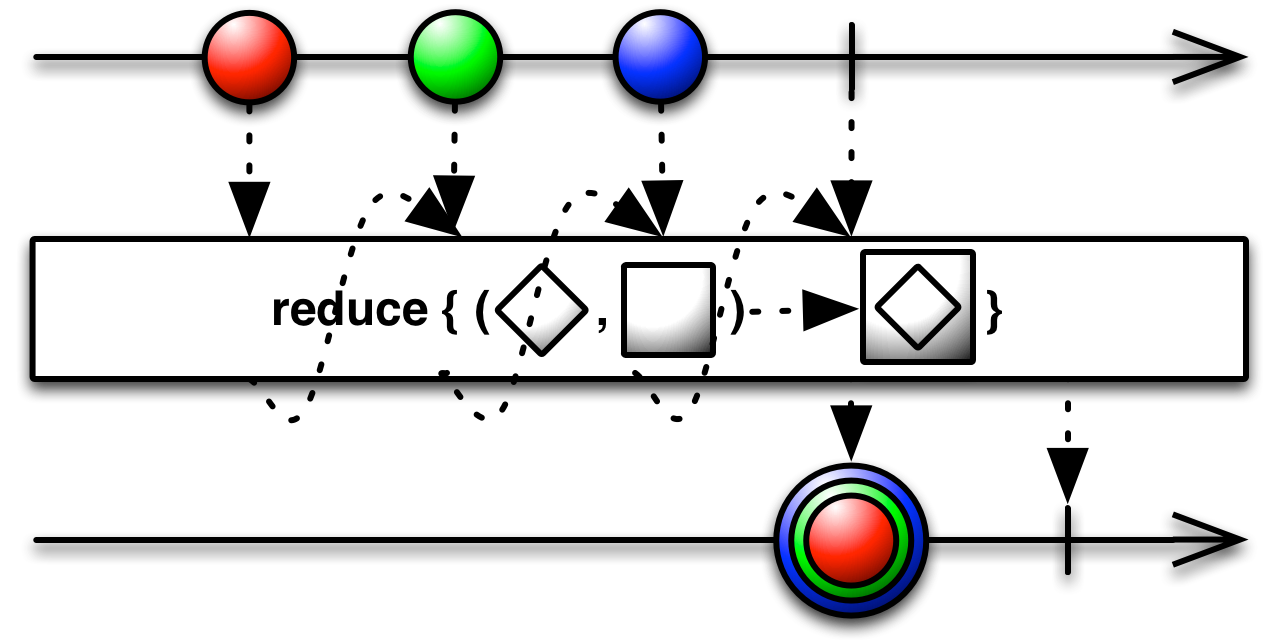
\includegraphics[height=2.5cm]{reduce.png}
  \end{center}

  Example: for \mintinline{scala}{Seq[String]}, reduction with string concatenation \mintinline{scala}{+} returns the concatenation of all the strings in the sequence.
\end{frame}

\begin{frame}[fragile]{Test failure: coarse types again}
  \inputminted[gobble=2]{console}{testQuick9.console}

  \begin{block}{Property-based testing revealed the \alert{unexpected}}
  \begin{itemize}
  \item Unexpected ambiguity:
    \begin{itemize}
    \item Intended behavior: output a number only if it has none of the divisors.
    \item Actual behavior: 1649349 is divisible by 13 but not 91, yet 1649349 was output.
    \end{itemize}
  \item Corner case: empty ``fizz'' and ``buzz'' words.
  \end{itemize}
  \end{block}
\end{frame}

\subsection{\mintinline{scala}{Option[A]} type}

\begin{frame}{An empty string is \alert{not} equivalent to no string}
  Presence of something ``empty'' is \alert{not} equivalent to the absence of something (contrary to how some programming languages work).

  \begin{itemize}
  \item Problem: special case condition, testing for an empty string, conflated an empty combined string with ``failed to be a multiple at all''.
  \item Solution: refine another \alert{type}!
  \end{itemize}
\end{frame}

\begin{frame}[fragile]{\mintinline{scala}{Option[A]} type}

  \mintinline{scala}{Option[A]} is one of two possibilities:
  \begin{itemize}
  \item \mintinline{scala}{None}
  \item \mintinline{scala}{Some(a)} wraps a value \mintinline{scala}{a} of type \mintinline{scala}{A}.
  \end{itemize}

  For example, \mintinline{scala}{Some("")} is not the same as \mintinline{scala}{None}.

  \begin{block}{Another Swift digression}
    Swift also has the option type, with special syntax.
  \end{block}

%  \inputminted{scala}{OptionExample1.scala}
\end{frame}

\begin{frame}[fragile]{Cleaning up the types}
  Change type \mintinline{scala}{Rule}:
  \inputminted[gobble=2]{scala}{FizzBuzz6.scala}

  Immediately get type errors:

  \inputminted[gobble=2]{console}{testQuick10.console}
\end{frame}

\begin{frame}[fragile]{Fix the type errors}

  \inputminted[gobble=2]{scala}{FizzBuzz7.scala}
\end{frame}

\begin{frame}[fragile]{Monoids}
  We define ``addition'' for \mintinline{scala}{Option[String]}:
  \inputminted[gobble=2]{scala}{FizzBuzz8.scala}
  
  \begin{block}{\mintinline{scala}{Option[String]} is a \href{http://en.wikipedia.org/wiki/Monoid}{Monoid}}
  \begin{itemize}
  \item There is an identity element (\mintinline{scala}{None}).
  \item There is a binary associative operator (\mintinline{scala}{addOption}).
  \end{itemize}
  \end{block}
\end{frame}

\section{Parallel \texttt{FizzBuzz}}

\begin{frame}[fragile]{Parallelism}
  \begin{itemize}
  \item Use of \alert{map}: parallelizable; there are high-performance \href{http://scala-blitz.github.io/}{parallel collections} for Scala.
  \item Use of \alert{reduce}: parallelizable because of the monoid property.
  \end{itemize}

  We discovered a theoretical speedup for generalized \texttt{FizzBuzz} from $O(n)$ to $O(\log n)$ (omitting some technical subtleties).

\end{frame}

\begin{frame}[fragile]{Parallelism (code)}
  \inputminted[gobble=2]{scala}{FizzBuzz9.scala}
\end{frame}

\section{Conclusion}

\begin{frame}{Conclusion}
  \begin{itemize}
  \item \alert{Tests} are useful.
  \item \alert{Types} are useful.
  \item Tests and types work well together to drive design and program evolution!
  \item Modern typed languages such as Scala promote fun, correct programming!
  \item It's a great time to be learning and using a modern typed language: Apple had good reasons to invent Swift.
  \end{itemize}

  \begin{block}{GitHub}
    All materials for this talk are available at \url{https://github.com/franklinchen/talk-on-type-directed-tdd-using-fizzbuzz}. The hyperlinks on the slide PDFs are clickable.
  \end{block}
\end{frame}

%\appendix


\end{document}

%%% Local Variables: 
%%% mode: latex
%%% TeX-master: "presentation"
%%% End: 
